%!TEX root = slides.tex

\section{Computational complexity}


\begin{frame}{Bubble sort for fixed size input}
  \begin{alertblock}{How many comparisons does bubble sort make for different inputs of the same size?}
    \begin{itemize}
      \item Suppose we have a list with 5 elements.
      \item Best case scenario: list already sorted.
      \item Worst case scenario: list reverse sorted.
    \end{itemize}
    \[ [1,2,3,4,5] \]
    \[ [5,2,1,4,3] \]
    \[ [5,4,3,2,1] \]
  \end{alertblock}
\end{frame}


\begin{frame}{Bubble sort different sized inputs}
  \begin{alertblock}{How many comparisons does bubble sort make for inputs of increasing length?}
    \begin{itemize}
      \item Suppose we have a list with $n$ elements.
      \item Compare the worst case scenario for each value of $n$.
    \end{itemize}
    \[ [3,2,1] \]
    \[ [4,3,2,1] \]
    \[ [5,4,3,2,1] \]
    \[ [6,5,4,3,2,1] \]
  \end{alertblock}
\end{frame}


\begin{frame}{Average vs. worst case}
  \begin{table}
    \begin{tabular}{p{2cm}rr}
      Input & Algorithm A & \hspace{1cm} Algorithm B \\
      \hline
      (1,2,3) &  1ms &  1ms \\
      (1,3,2) &  1ms &  5ms \\
      (2,1,3) &  2ms &  4ms \\
      (2,3,1) &  2ms &  5ms \\
      (3,1,2) &  2ms &  5ms \\
      (3,2,1) & 10ms &  4ms \\
      \hline
      Average &  3ms &  4ms \\
      Worst   & 10ms &  5ms
    \end{tabular}
  \end{table}
  \begin{center}
    Would you choose Algorithm A or Algorithm B?
  \end{center}
\end{frame}


\begin{frame}{Terminology of complexity}
  \begin{alertblock}{How does the number of operations change as $n$ increases?}
    \begin{description}
      \item[Linear] Multiply $n$ by a constant, add a constant. (Special category of polynomial time.)
      \item[Polynomial] Multiply $n$ by itself a fixed number of times, multiply by a constant. (Can add such terms together.)
      \item[Exponential] Raise a constant to the power of $n$. (Rate of change is still exponential.)
      \item[Logarithmic] Opposite of exponential.
    \end{description}
  \end{alertblock}
\end{frame}


\begin{frame}[fragile]{Terminology of complexity (graph)}
\begin{center}
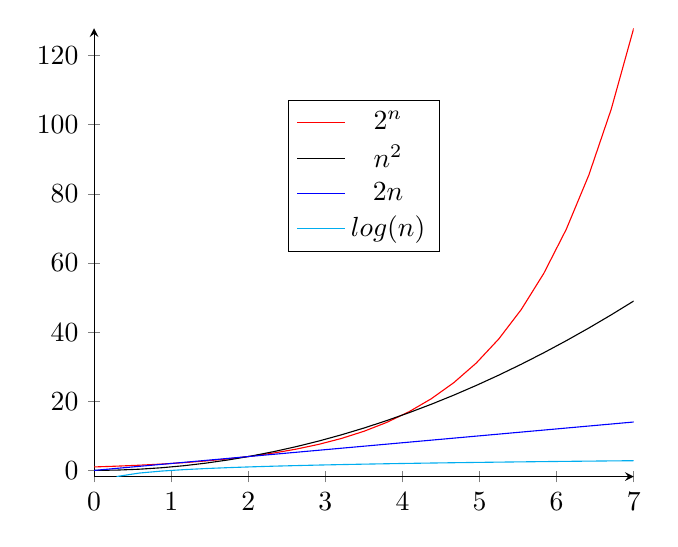
\begin{tikzpicture}
  \begin{axis}[xmin=0, domain=0:7, axis x line=bottom, axis y line=left, legend style={at={(0.5,0.5)},anchor=south}]
    \addplot[red]   {pow(2,x)};
    \addplot[black] {pow(x,2)};
    \addplot[blue]  {2*x};
    \addplot[cyan]  {ln(x)/ln(2))};
    \legend{$2^n$,$n^2$,$2n$,$log(n)$};
  \end{axis}
\end{tikzpicture}
\end{center}
\end{frame}



\begin{frame}{Linear}
  \[ f(n) = a_0 + a_1 n \]
  \begin{alertblock}{How many pairs of shoes does a centipede need?}
    \begin{itemize}
      \item Let's say a centipede has 100 feet.
      \item Then every centipede needs 100 shoes.
      \item That's 50 pairs of shoes.
      \item So 2 centipedes need 100 pairs, 3 need 150 pairs, etc.
      \item So $n$ centipedes need $50n$ pairs of shoes.
      \item Linearity is familiar, and most people's default assumption.
      \item You take the input, multiply by a constant, and add another constant.
    \end{itemize}
  \end{alertblock}
\end{frame}


\begin{frame}{Polynomial}
  \[ f(n) = a_0 + a_1 n + a_2 n^2 + a_3 n^3 + \ldots \]
  \begin{alertblock}{What is the volume of a cube of side $n$?}
    \begin{itemize}
      \item Suppose we have a cube with sides of length 1 metre.
      \item The volume of the cube is $1 \times 1 \times 1 = 1$ metres cubed.
      \item Suppose the cube has sides of length 2 metres instead.
      \item The volume of the cube is $2 \times 2 \times 2 = 8$ metres cubed.
      \item In general, for sides of length $n$, the volume is $n^3$.
    \end{itemize}
  \end{alertblock}
\end{frame}


\begin{frame}{Exponential}
  \[ f(n) = a^n \]
  \begin{alertblock}{How many numbers can we represent with $n$ bits?}
    \begin{itemize}
      \item Consider the case of four bits -- imagine four placeholders \textbf{\fbox{?}}\textbf{\fbox{?}}\textbf{\fbox{?}}\textbf{\fbox{?}}
      \item Each placeholder can contain either 0 or 1.
      \item There are $2 \times 2 \times 2 \times 2 = 2^4 = 16$ different numbers.
      \item Add another bit, how many numbers is it now?
      \item It's $2 \times 2 \times 2 \times 2 \times 2 = 2^5 = 32$.
      \item Generally $n$ bits can represent $2^n$ numbers.
    \end{itemize}
  \end{alertblock}
\end{frame}

\begin{frame}{Logarithmic}
  \[ f(n) = log_a n \]
  \begin{alertblock}{How many bits do we need to represent $n$ numbers?}
    \begin{itemize}
      \item If we have $n$ bits we can represent $2^n$ numbers.
      \item If we want to represent $n$ numbers, how many bits to we need (at a minimum)?
      \item The inverse operation to exponentiation is logarithm.
      \item Remember, $a^n = b$ means $log_a b = n$.
    \end{itemize}
  \end{alertblock}
\end{frame}




\begin{frame}{Polynomial time}
  \begin{definition}
  An algorithm is said to be solvable in \emph{polynomial time} if the number of steps required to complete the algorithm for a given input is $O(n^k)$ for some nonnegative integer $k$, where $n$ is the complexity of the input.
  \end{definition}
  
  \vspace{0.5cm}
  \metroset{block=fill}
  \begin{block}{$P$ complexity class}
  The $P$ complexity class is the set of problems for which there exists, for each such problem, at least one algorithm to solve that problem in polynomial time.
  \end{block}

  \citeurl{mathworld.wolfram.com/P-Problem.html}
\end{frame}



\begin{frame}{Polynomial time on a Turing machine}
  \begin{description}
    \item[Sorting] algorithms are usually compared in terms of comparisons.
    \item[Other algorithms] might be compared in terms of something else, like iterations.
    \item[With Turing machines] we can use the number of times we look up the state table.
    \item[The size] of the input can be the length of the input on the tape initially.
  \end{description}
\end{frame}




\begin{frame}{Recap on Languages}
  \begin{description}
    \item[Alphabet] Finite set of symbols, denoted $\Sigma$.
    \item[String] Sequence of symbols, $w$ from $\Sigma$.
    \item[Language] Set of strings, denoted $L$.
    \item[Length] Of a string, denoted $|w|$  .
    \item[Empty string] Unique string of length 0, denoted $\epsilon$.
  \end{description}
\end{frame}


\begin{frame}{Kleene star}
  \begin{description}
    \item[Word concatenation:] $w_1 w_2$ is the concatenation of strings $w_1$ and $w_2$.
    \item[String concatenation:] $L_1 L_2$ is the language resulting from the concatenation of all strings in $L_1$ and all words in $L_2$, in that order.
    \item[Powers:] $L^0 = \{ \lambda \}$, $L^1 = L$ and $L^{n+1} = L^n L$ for all $n > 1$.
  \end{description}
  
  \vspace{0.5cm}
  
  \begin{block}{Kleene Star}
     \[ L^* =  \bigcup_{i=0}^{\infty} L^i \]
  \end{block}
  
  Note that treating the alphabet $\Sigma$ as a language in itself, we get that $\Sigma^*$ is the set of all words over $\Sigma$.
\end{frame}


\begin{frame}{Example}
  \begin{description}
    \item[$\Sigma$] $\{ 0, 1 \}$
    \item[$L$] $\{ 00, 01, 10, 11 \}$
    \item[$w_1$] $01$
    \item[$w_3$] $11$
    \item[$w_1 w_3$] $0111$
    \item[$\Sigma^*$] $\{ \lambda, 0, 1, 00, 01, 10, 11, 001, 010, \ldots \}$
    \item[$L^*$] $\{ \lambda, 00, 01, 10, 11, 0000, 0001, \ldots \}$
    \item[$L^+$] $\{ 00, 01, 10, 11, 0000, 0001, \ldots \}$
  \end{description}
\end{frame}










\begin{frame}{Non-deterministic polynomial time}
  \begin{definition}
  A problem is in the $NP$ complexity class if it is solvable by a non-deterministic Turing Machine in polynomial time. A non-deterministic Turing Machine is one which may not have a unique action to take for some or all states and inputs.
  \end{definition}
  
  \vspace{0.5cm}
  \metroset{block=fill}
  \begin{block}{$P$ is a subset of $NP$}
  The $P$ complexity class is a subset of $P$ because all polynomial time solvabled problems can be modelled using Nondeterministic Turing Machinses.
  \end{block}

  \citeurl{mathworld.wolfram.com/P-Problem.html}
\end{frame}


\begin{frame}{Decision problems}
  \begin{description}
    \item[Decision problems] are problems where the answer is 0 or 1.
    \vspace{0.5cm}
    \item[Restricting] ourselves to decision problems is convenient and fair.
    \vspace{0.5cm}
    \item[$f:\{0,1\}^n \rightarrow \{0,1\}$] is useful notation for considering decision problems.
    \vspace{0.5cm}
    \item[Other problems] can be easily (polynomial time) adapted into decision problems.
  \end{description}
\end{frame}
